\documentclass[10pt, a5paper]{article}
\usepackage{pdfpages}
\usepackage{parallel}
\usepackage[T2A]{fontenc}
\usepackage{ucs}
\usepackage[utf8x]{inputenc}
\usepackage[polish,english,russian]{babel}
\usepackage{hyperref}
\usepackage{rotating}
\usepackage[inner=2cm,top=1.8cm,outer=2cm,bottom=2.3cm,nohead]{geometry}
\usepackage{listings}
\usepackage{graphicx}
\usepackage{wrapfig}
\usepackage{longtable}
\usepackage{indentfirst}
\usepackage{array}
\newcolumntype{P}[1]{>{\raggedright\arraybackslash}p{#1}}
\frenchspacing
\usepackage{fixltx2e} %text sub- and superscripts
\usepackage{icomma} % коскі ў матэматычным рэжыме
\PreloadUnicodePage{4}

\newcommand{\longpage}{\enlargethispage{\baselineskip}}
\newcommand{\shortpage}{\enlargethispage{-\baselineskip}}

\def\switchlang#1{\expandafter\csname switchlang#1\endcsname}
\def\switchlangbe{
\let\saverefname=\refname%
\def\refname{Літаратура}%
\def\figurename{Іл.}%
}
\def\switchlangen{
\let\saverefname=\refname%
\def\refname{References}%
\def\figurename{Fig.}%
}
\def\switchlangru{
\let\saverefname=\refname%
\let\savefigurename=\figurename%
\def\refname{Литература}%
\def\figurename{Рис.}%
}

\hyphenation{admi-ni-stra-tive}
\hyphenation{ex-pe-ri-ence}
\hyphenation{fle-xi-bi-li-ty}
\hyphenation{Py-thon}
\hyphenation{ma-the-ma-ti-cal}
\hyphenation{re-ported}
\hyphenation{imp-le-menta-tions}
\hyphenation{pro-vides}
\hyphenation{en-gi-neering}
\hyphenation{com-pa-ti-bi-li-ty}
\hyphenation{im-pos-sible}
\hyphenation{desk-top}
\hyphenation{elec-tro-nic}
\hyphenation{com-pa-ny}
\hyphenation{de-ve-lop-ment}
\hyphenation{de-ve-loping}
\hyphenation{de-ve-lop}
\hyphenation{da-ta-ba-se}
\hyphenation{plat-forms}
\hyphenation{or-ga-ni-za-tion}
\hyphenation{pro-gramming}
\hyphenation{in-stru-ments}
\hyphenation{Li-nux}
\hyphenation{sour-ce}
\hyphenation{en-vi-ron-ment}
\hyphenation{Te-le-pathy}
\hyphenation{Li-nux-ov-ka}
\hyphenation{Open-BSD}
\hyphenation{Free-BSD}
\hyphenation{men-ti-on-ed}
\hyphenation{app-li-ca-tion}

\def\progref!#1!{\texttt{#1}}
\renewcommand{\arraystretch}{2} %Іначай формулы ў матрыцы зліпаюцца з лініямі
\usepackage{array}

\def\interview #1 (#2), #3, #4, #5\par{

\section[#1, #3, #4]{#1 -- #3, #4}
\def\qname{LVEE}
\def\aname{#1}
\def\q ##1\par{{\noindent \bf \qname: ##1 }\par}
\def\a{{\noindent \bf \aname: } \def\qname{L}\def\aname{#2}}
}

\def\interview* #1 (#2), #3, #4, #5\par{

\section*{#1\\{\small\rm #3, #4. #5}}

\def\qname{LVEE}
\def\aname{#1}
\def\q ##1\par{{\noindent \bf \qname: ##1 }\par}
\def\a{{\noindent \bf \aname: } \def\qname{L}\def\aname{#2}}
}


\begin{document}

\title{Amazon auto-scaling. Создание и оптимизация автомасштабируемых систем на базе Linux}
\author{Виктор Краев\footnote{Минск, Беларусь, \url{anakreon.by}}}
\date{}
\maketitle
\begin{abstract}\noindent 
The technology of auto-scaling clasters provided by Amazon for its cloud services is reviewed. Approach to monitor and control such cloud-based system is presented, as far as practical expe\-ri\-ence of migrating to the auto-scaled services.
\end{abstract}

\section*{Amazon EC2. Cloud vs Hardware}
С каждым годом IT-индустрия набирает обороты, но как бы не развивались технологии, ресурс выработки железа пока никто не победил. Отказ оборудования по-прежнему является одной из главных проблем современного хостинга. Конечно же, всегда есть возможность создания избыточности, но это тянет за собой достаточно серьезные расходы на дополнительное оборудование и его обслуживание. Поэтому наша компания обратила внимание на облачные вычисления. Наиболее продвинутой компанией, способной решить наши задачи, на сегодняшний день оказалась Amazon. Хотя их технология Elastic Cloud --- местами сырая, она находится в активной разработке и интегрируется с другими сервисами, нивелирующими ее недостатки. Не победив проблему «железа», в Amazon создали избыточность, покрыв недостатки другими сервисами, и сегодня падение инстансов (instances) или потеря данных в облаке иногда присутствует, но успешно компенсируется резервным копированием и высокой скоростью создания инстансов из резервных копий. Интеграция с такими сервисами, как auto-scaling, cloudwatch, cloudformation, позволяет добиться избыточности, намного превышающей возможности обычного кластера серверов, не задумываясь о «железе».  

\section*{Amazon Auto-Scaling. Hardware cluster vs scalable cloud}

На сегодняшний день для увеличения доступности и избыточности ресурса используют технологии кластеризации. Статический кластер подразумевает под собой использование определенного неизменяемого количества (больше 1) серверов, нагрузку между которыми распределяет балансировщик (Load Balancer). Это хорошее решение для ресурсов с постоянно высокой нагрузкой. Динамический кластер --- это кластер, где распределение нагрузки осуществляется между серверами, количество которых может меняться в зависимости от нужд и нагруженности проекта. Однако в «железе» это трудноосуществимо, т.к. тянет за собой целый шлейф проблем, связанных с установкой оборудования, разворачиванием ПО, а главное --- времени. С помощью сервиса EC2 на создание виртуального сервера уходит несколько минут. Создание происходит из уже готового образа (image), т.~е. выполняется клонирование существующей системы. Обычно это образы «чистых» систем, в которых установлены лишь базовые пакеты. Но Amazon позволяет создавать собственные образы уже настроенных и готовых к использованию систем --- например, хостинговых. Полученные образы помещаются в приватное хранилище, из которого в любой момент можно создать и отправить в работу клон. Эта технология, лежащая в основе создания динамического кластера и известная как AMI, позволяет мгновенно создавать кластеры различного размера. Для распределения нагрузки между элементами кластера используется сервис ELB (Elastic Load Balancer), который позволяет менять размерность кластера путем добавления или удаления виртуальных серверов в балансировщик. Однако, используя лишь web-интерфейс, вы сможете управлять кластером только вручную. Это значит, что если один из элементов кластера откажет в обслуживании, то балансировщик выбросит его из пула обрабатываемых запросов, и новый виртуальный сервер не встанет на его место автоматически. Чтобы автоматизировать этот процесс в Amazon придумали технологию Auto-Scaling. Эта технология позволяет задавать размерность кластера и использует проверку здоровья (health cheacking) серверов из ELB или EC2. В случае падения на место упавшего сервера из образа автоматически создается новый сервер и добавляет его в балансировщик. Сегодня управление конфигурацией Auto-Scaling осуществляется только через API, что позволяет автоматизировать процессы создания кластеров и управления ими, убирая из цепочки слабое звено "--- человека.

\section*{Amazon CloudWatch. Monitor and automate your systems}

Мы можем не только управлять собственной армией виртуальных серверов, но и получать данные о ее работе. Технология \linebreak CloudWatch позволяет осуществлять мониторинг. В основе этой технологии лежат метрики (metrics) "--- данные, собираемые с инстансов и агрегируемые по различным критериям в группы. Нельзя сказать, что технология блещет богатством собираемых коллекций, хотя в ней присутствует мониторинг CPU, дисковой и сетевой подсистем, количества запросов в ELB и т.\,д. Но с помощью API вы можете собирать свою собственную коллекцию метрик, которую в дальнейшем сможете использовать для автоматизации некоторых процессов. Автоматизация на основе метрик --- главное предназначение этого сервиса. Кроме сбора статистики, этот сервис может ее обрабатывать и выполнять на основе полученных результатов определенные действия. В простейшем случае это отправка сообщения о превышении ранее выставленного порога. Кроме того, на определенное событие, полученное в ходе обработки метрик, можно прикрутить действия с Auto-Scaling, что дает возможность построения автоматически масштабируемыех кластеров. 

Рассмотрим пример создания действия автомасштабирования с помощью API. Пусть требуется создать автомасштабируемый кластер --- группу инстансов, обслуживаемых одним балансировщиком с минимальным количеством 1 и максимальным 7, которая меняет количество задействованных в распределении запросов на web-сервер в зависимости от нагрузки на процессор. Для этого мы создаем AMI-образ из инстанса, который мы хотим масштабировать. С помощью команды as-create-launch-config из AS API создаем конфигурацию, в которой указываем тип инстанса и ID нашего образа. После этого с помощью команды as-create-auto-scaling-group создаем группу, в параметрах которой указываем название нашего launch config, минимальный и максимальный размер группы, название ELB-балансировщика (который мы создали заранее). После этих действий кластер готов. Теперь необходимо интегрировать нашу AS-группу с сервисом CloudWatch. Для этого создаем 2 политики с помощью команды as-put-scaling-policy. Первая политика UP1 добавляет 1 инстанс в группу, вторая DOWN1 --- удаляет 1 инстанс. Дальше, используя сервис CloudWatch (через web-интерфейс или API), создаем 2 обработчика событий: 
\begin{enumerate}
	\item При взлете выше среднего порогового значения 80\% CPU за 5 минут --- использовать политику UP1. 
	\item При падении ниже среднего порогового значения 20\% CPU за 5 минут --- использовать политику DOWN1. 
\end{enumerate}
Теперь кластер будет сам себя масштабировать, полагаясь на данные метрики CPU, агрегированной по нашей группе. 

\section*{Nginx + Memcached over LUA. Cache and distribute}

Технология автомасштабирования великолепно работает и решает повседневные задачи, обеспечивая бесперебойную работу интернет"=ресурсов. Мы убедились в этом, осуществив миграцию интернет"=ресурса \url{theuptake.org} в облако Amazon. Прежний кластер из 8 серверов стал автомасштабируемой системой. В обычном режиме на данный момент работает 1 small instance (самый дешевый виртуальный сервер), который в случае увеличения нагрузки масштабируется в течение нескольких минут до стабильного состояния между средними пороговыми значениями метрик CloudWatch. Однако, путь в динамическому масштабированию оказался не так прост, как использованиесервисов Amazon. Интернет-ресурс построен на движке Wordpress, который очень ресурсоемкий и требует значительного количества процессорного времени на обработку PHP"=кода. Существует несколько кэширующих плагинов, решающих эту проблему, и мы опробовали их все. Из них можно выделить 2 мощных решения:  WP Super Сache и WC3 Total Cache. Однако и для них результаты оказались недостаточными для динамического кластера. Самый быстрый "--- WP Super Сache. Он помещает сгенерированные страницы в файловую систему и (например, с помощью Nginx и реврайтов) позволяет отдавать контент с по-настоящему высокими скоростями. Однако его использование порождает 2 проблемы: 
\begin{enumerate}
	\item Каждый инстанс хранит свой уникальный кэш. 
	\item При добавлении нового инстанса в кластер кэш отсутствует, и требуется время на его генерацию, что в условиях быстро увеличивающейся нагрузки хоронит его под прессом запросов. 
\end{enumerate}

Плагин WC3 Total Cache, как и WP Super Сache, может хранить кэш в файловой системе, но умеет складывать страницы (и даже SQL-запросы) в memcached "--- общее для всех инстансов хранилище. Это решает проблему инвалидации и прегенерации кэша, но, скорости оказываются очень далеки от идеала. Если раньше ресурсы уходили на генерацию кода, то в данном случае они уходят на обслуживания системы кэширования, которая исполняется на том же самом PHP. Поэтому было принято решение сделать систему кэширования без использования PHP и связать Nginx напрямую с Memcached, исключив таким образом PHP из управления кэшем. Для реализации этой идеи потребовались Memcached и Nginx с модулями lua-nginx-module, memc-nginx-module, ngx\_devel\_kit,  ngx\_http\_upstream\_keepalive, set-misc-nginx-module, srcache-nginx-module. С помощью этого ПО автором была реализована приведенная на рис. схема.

\begin{figure}[ht]
\centering{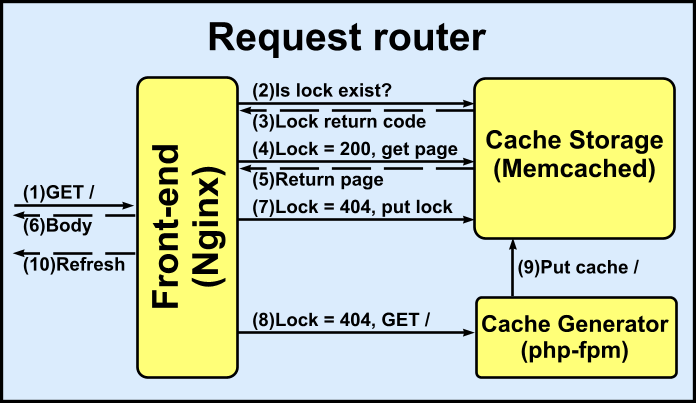
\includegraphics[width=8cm]{14_kraev.png}}
\label{pic:kraev}
%\caption{Приложения по категориям}
\end{figure}

По этой схеме Nginx выступает в качестве маршрутизатора между хранилищем кэша и кэш-генератором, вызывая для обработки запросов LUA-скрипт. Таким образом, страницы всегда отдаются из кэша. Если же кэша не существует, отправляется запрос для его генерации, а клиент перенаправляется на refresh-страницу, которая заставляет отправить запрос повторно через заданное время. Кэш имеет expire time = 0, что означает,  что он никогда не будет удален. Для обновления кэша используется lock с ограниченным expire time (в зависимости от запрашиваемой страницы), и когда expire time истекает "--- кэш регенерируется и помещается поверх старого. Также lock имеет еще одну важную функцию: его наличие предотвращает отправку запросов на генерацию из других фронтендов, если  автомасштабируемый кластер стал раздуваться, и в группе находится больше одного инстанса. 

Общее хранилище решает проблему прегенерации кэша. Так, при добавлении нового инстанса, он сразу вступает в распределение нагрузки, используя кэш из общего хранилища.  Такой подход позволяет ускорить ресурсы не только с Wordpress, а в принципе любой ресурс с ПО, написанным на любом коде, из которого генерируется HTML.

\section*{Save and profit!}

Использование данных технологий позволило нашей компании существенно снизить затраты на техническое обеспечение интернет-ресурса \url{theuptake.org}. Заменив 8 физических серверов (80--90\% времени они простаивали, но были необходимы из-за периодических резких всплесков посещений после публикации новостей), на 1 large-инстанс, на котором хранится общий контент и кэш, 1 RDS-инстанс, в котором лежит БД и автомасштабируемая группировка, работающая во время простоя с 1 smallинстанса и раздуваемая до кластера, размер которого определяет нагрузка. В дополнение к экономии (т.к. сегодня мы платим только за пики) мы многократно повысили скорость отдачи контента,  доступность и отказоустойчивость ресурса. 

\end{document}
